\chapter{Vector Basics}
    \section{Recommended Texts}
        The following books are recommended for the course. The first one will be followed by the instructor.
        \begin{enumerate}
            \item Engineering Electromagnetics 8th Edition by John Buck \& William H. Hayt
            \item Electromagnetics John D. Kraus
            \item Introduction to Electrodynamics by David J. Griffiths
            \item Classical Electrodynamics by John David Jackson
        \end{enumerate}
    \section{What is a Vector?}
        From a mathematical standpoint a vector is an element of a vector space. From a physical point of view a vector is a quantity that requires a magnitude as well as a direction to be represented.
    \section{Unit vectors in Rectangular Coordinate System}
        In a Rectangular Coordinate System (RCS), a vector can be represented as a linear sum of three unit vectors, namely $\vec{a}_x$, $\vec{a}_y$ and $\vec{a}_z$. In case of two dimensions, $\vec{a}_z$ is not needed. This is also depicted in figure~\ref{fig:vectors}.
        \begin{figure}
            \centering
            \subfloat[A vector in two dimensions]{
                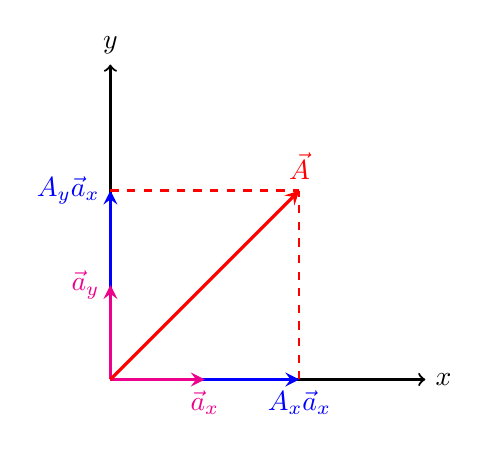
\begin{tikzpicture}
    [scale=4,
    axis/.style={->,thick},
    vector/.style={-stealth,very thick},
    vector guide/.style={dashed,red,thick}]

    \coordinate (O) at (0, 0);
    \def\u{0.3}
    \def\v{0.6}

    % drawing axes
    \draw[axis] (O) -- (1, 0) node[anchor=west]{$x$};
    \draw[axis] (O) -- (0, 1) node[anchor=south]{$y$};

    % drawing the vector's components
    \draw[vector, blue] (O) -- (\v, 0) node[anchor=north]{$A_x\vec{a}_x$};
    \draw[vector, blue] (O) -- (0, \v) node[anchor=east]{$A_y\vec{a}_x$};

    % drawing unit vectors
    \draw[vector, magenta] (O) -- (\u, 0) node[anchor=north]{$\vec{a}_x$};
    \draw[vector, magenta] (O) -- (0, \u) node[anchor=east]{$\vec{a}_y$};

    % drawing vector A
    \draw[vector, red] (O) -- (\v, \v) node[anchor=south]{$\vec{A}$};

    % drawing vector guides
    \draw[vector guide] (\v, 0) -- (\v, \v);
    \draw[vector guide] (0, \v) -- (\v, \v);

\end{tikzpicture}
            }
            \subfloat[A vector in three dimensions]{
                % sets up the perspective from which we are looking at the picture {theta}{phi}
% {theta} defines the rotion by x axis while {phi} defines the rotation by z axis
\tdplotsetmaincoords{60}{120}

\begin{tikzpicture}
    [scale=4,
    tdplot_main_coords,
    axis/.style={->,black,thick},
    vector/.style={-stealth,very thick},
    vector guide/.style={dashed,red,thick}]

    \coordinate (O) at (0, 0, 0);

    % this should serve as our unit vector
    \def\u{0.3} 
    \def\v{0.6}
    % drawing axes
    \draw[axis] (0, 0, 0) -- (1, 0, 0) node[anchor=north east]{$x$};
    \draw[axis] (0, 0, 0) -- (0, 1, 0) node[anchor=north west]{$y$};
    \draw[axis] (0, 0, 0) -- (0, 0, 1) node[anchor=south]{$z$};

    % drawing the components of the vector A: Drawing them first so the unit vectors do appear
    \draw[vector, blue] (O) -- (\v, 0, 0) node[anchor=south east]{$B_x\vec{a}_x$};
    \draw[vector, blue] (O) -- (0, \v, 0) node[anchor=south west]{$B_y\vec{a}_y$};
    \draw[vector, blue] (O) -- (0, 0, \v) node[anchor=south east]{$B_z\vec{a}_z$};

    % drawing the unit vectors
    \draw[vector, magenta] (O) -- (\u, 0, 0) node[anchor=south east]{$\vec{a}_x$};
    \draw[vector, magenta] (O) -- (0, \u, 0) node[anchor=south west]{$\vec{a}_y$};
    \draw[vector, magenta] (O) -- (0, 0, \u) node[anchor=east]{$\vec{a}_z$};

    % drawing the main vector B
    \draw[vector, red] (O) -- (\v, \v, \v) node[anchor=south east]{$\vec{B}$};

    % projection on xy axis
    \draw[vector guide] (\v, 0, 0) -- (\v, \v, 0);
    \draw[vector guide] (0, \v, 0) -- (\v, \v, 0);
    \draw [vector guide] (\v, \v, 0) -- (\v, \v, \v);

    % drawing projection on yz axis
    \draw[vector guide] (0, \v, 0) -- (0, \v, \v);
    \draw[vector guide] (0, 0, \v) -- (0, \v, \v);
    \draw[vector guide] (0, \v, \v) -- (\v, \v, \v);

    % drawing projection on xz axis
    \draw[vector guide] (0, 0, \v) -- (\v, 0, \v);
    \draw[vector guide] (\v, 0, 0) -- (\v, 0, \v);
    \draw[vector guide] (\v, 0, \v) -- (\v, \v, \v);


\end{tikzpicture}
            }
            \caption{}
            \label{fig:vectors}
        \end{figure}
    \section{Dot Product}
        Suppose we have two vectors $\vec{A}$ and $\vec{B}$. $\vec{A}$ can be represented as:
        $$\vec{A} = A_x\vec{a}_x + A_y\vec{a}_y + A_z\vec{a}_z$$
        Similarly, $\vec{B}$ can be represented as:
        $$\vec{B} = B_x\vec{a}_x + B_y\vec{a}_y + B_z\vec{a}_z$$
        Their dot product, $\vec{A}\cdot \vec{B}$, which is a scalar quantity, is defined as:
        \begin{equation}\label{eq:dotproductfirst}
            \vec{A}\cdot \vec{B} = |\vec{A}||\vec{B}|\cos \theta
        \end{equation}
        In case when $\theta$ becomes $90^{\circ}$ the dot product automatically reduces to zero. Thus one can easily conclude that the dot product of two perpendicular vectors shall always be zero. This makes expressing the dot product in terms of its components pretty straight forward.
        $$\vec{A}\cdot \vec{B} = \left(A_x\vec{a}_x + A_y\vec{a}_y + A_z\vec{a}_z\right)\cdot \left(B_x\vec{a}_x + B_y\vec{a}_y + B_z\vec{a}_z\right)$$
        \begin{equation}\label{eq:dotproduct}
           \vec{A}\cdot \vec{B} = A_xB_x + A_yB_y + A_zB_z
        \end{equation}
        A vector can also be represented in the form of column vector as:
        $$ \vec{A} = \begin{bmatrix}A_x \\A_y \\A_z\\ \end{bmatrix} \quad \vec{B} = \begin{bmatrix}B_x \\B_y \\B_z\\ \end{bmatrix} $$
        In that case the dot product, also called inner product in this context, is defined as:
        $$ \mathbf{A}^{T}\mathbf{B} $$
        If the vectors $\vec{A}$ and $\vec{B}$ are of the order $n \times 1$ their inner product will have the order $ 1 \times \left(n \times n\right) \times 1 = 1 \times 1$. Thus the result will be a scalar quantity.
        The opposite of the inner product is known as the outer product also called the cross product which we will get to in a later topic.
        
        \subsection{Cauchy Bunyakovsky Schwarz Inequality}
            The theorem states:
            $$|\vec{A}\cdot \vec{B}| \leq |\vec{A}||\vec{B}|$$
            It's easy to see why this is the case by replacing $\vec{A}\cdot \vec{B}$ by it's value:
            $$|\vec{A}||\vec{B}|\cos \theta \leq |\vec{A}||\vec{B}| $$
            This inequality changes to an equality when both vectors are collinear.
        
        \subsection{The Triangle Inequality}
            $$|\vec{A}| + |\vec{B}| \geq |\vec{A} + \vec{B}| $$
            It's quite easy to see why that is the case in the case of two dimensions.
            At this moment it should be useful to point out that:
            $$|\vec{A}| = \sqrt{A_x^2 + A_y^2 + A_z^2}$$
            $$|\vec{A}|^2 = \vec{A} \cdot \vec{A}$$
            This shall be useful in proving the Parallelogram Equality.
        
        \subsection{The Parallelogram Equality}
            The equality states:
            $$|\vec{A} + \vec{B}|^2 + |\vec{A} - \vec{B}|^2 = 2\left(|\vec{A}|^2+\vec{B}^2\right)$$
            To prove it:
            $$|\vec{A} + \vec{B}|^2 = \left(\vec{A}+\vec{B}\right)\cdot \left(\vec{A}+\vec{B}\right)$$
            $$= \vec{A}\cdot \vec{A} + \vec{A}\cdot \vec{B} + \vec{B}\cdot \vec{A} + \vec{B}\cdot \vec{B}$$
            $$= |\vec{A}|^2 -2\vec{A}\cdot \vec{B} + |\vec{B}|^2$$
            Similarly:
            $$|\vec{A} - \vec{B}|^2 = \left(\vec{A}-\vec{B}\right)\cdot \left(\vec{A}-\vec{B}\right)$$
            $$= \vec{A}\cdot \vec{A} - \vec{A}\cdot \vec{B} - \vec{B}\cdot \vec{A} + \vec{B}\cdot \vec{B}$$
            $$= |\vec{A}|^2 +2\vec{A}\cdot \vec{B} + |\vec{B}|^2$$
            Thus:
            $$|\vec{A} + \vec{B}|^2 + |\vec{A} - \vec{B}|^2 = 2|\vec{A}| + 2|\vec{B}| = 2\left(|\vec{A}| + |\vec{B}|\right)$$
        
        \subsection{Scalar component of one vector in the direction of another}
            \begin{figure}
    \centering
    \begin{tikzpicture}
        [scale=6,
        axis/.style={->,thick},
        vector/.style={-stealth,very thick},
        vector guide/.style={dashed,red,thick}]

        \def\ang{45}

        \draw (0, 0) node[left]{$O$};
        % drawing both vectors and their angle's arc
        \draw[vector, blue] (0, 0) -- (0.5, 0) node[anchor=north]{$\vec{A}$};
        \draw[vector, red] (0, 0) -- (\ang: 0.5) node[anchor=south]{$\vec{B}$};
        \draw[black] (0.1, 0) arc (0:\ang:0.1);
        \draw (30: 0.1) node[right]{$\theta$};

        % dropping a perpendicular from B's tip to A
        \draw[dashed] (\ang: 0.5) -- ($(0,0)!(\ang: 0.5)!(1, 0)$) node[below]{$P$};

        % dropping a perpendicular from A's tip to B
        \draw[dashed] (0.5, 0) -- ($(0,0)!(0.5, 0)!(\ang: 0.5)$) node[left]{$Q$};

    \end{tikzpicture}
    \caption{Projections of two vectors $\vec{A}$ and $\vec{B}$ on each other.}
    \label{fig:projectiontwovectors}
\end{figure}
            Dot product can be really handy when we want to figure out the projection of one vector onto the direction of another vector. Refer to figure\ref{fig:projectiontwovectors}. The line $\bar{OP}$ is the projection of vector $\vec{B}$ in the direction of $\vec{A}$. Similarly, $\bar{OQ}$ is the projection of vector $\vec{A}$ in the direction of vector $\vec{B}$. Since the line from the tip of vector $\vec{B}$ to $P$ is perpendicular to the vector $\vec{A}$ and the line from the tip of $\vec{A}$ to point $Q$ is perpendicular to vector $\vec{B}$. We can apply trigonometry to find out these projections. 

            \noindent Let $B_A$ denote the projection of vector $\vec{B}$ in the direction of $\vec{A}$ and let $A_B$ denote the projection of $\vec{A}$ in the direction of $\vec{B}$. Applying trigonometry we get:
            $$B_A = |\vec{B}|\cos\theta$$
            $$A_B = |\vec{A}|\sin\theta$$
            Recalling the definition of a dot product from equation~\ref{eq:dotproductfirst} we can see:
            $$B_A = \frac{\vec{A}\cdot\vec{B}}{|\vec{A}|} = \vec{u}_A\cdot\vec{B}$$
            $$A_B = \frac{\vec{A}\cdot\vec{B}}{|\vec{B}|} = \vec{u}_B\cdot\vec{A}$$
        
        \subsection{Some practical applications}
            Some common places in Physics where you will find the dot product being applied are:
            \begin{itemize}
                \item The formulas for work done.
                        $$W = \vec{F}\cdot \vec{d}$$ 
                        $$dW = \vec{F}\cdot \vec{dl}$$
                        $$W = \int\limits_{L} \vec{F}\cdot \vec{dl}$$
                \item The forumulas for Electric and Magnetic flux.
                        $$\phi_E = \vec{E}\cdot \vec{A}$$
                        $$\phi_M = \vec{B}\cdot \vec{A}$$
                \item A third one I don't understand yet. Need to confirm this one.
                        $$Q = \iint\limits_{S}\vec{D}\cdot \vec{dS}$$
            \end{itemize}
    \section{Cross Product}
        \subsection{The Definition}
            The cross product of two vectors $\vec{A}$ and $\vec{B}$ is given by:
            \begin{equation}\label{eq:crossproduct}
                \vec{A}\times \vec{B} = |\vec{A}||\vec{B}|\sin\theta \vec{u}_N
            \end{equation}
            Where $\theta\in\left[0, \pi\right]$ and $\vec{u}_N$ is a vector given by the right hand rule where fingers should be curled from the direction of $\vec{A}$ to the direction of $\vec{B}$.
            Since the direction of the cross product is dictated by the right hand rule we can already see that it is not a commutative operation. More accurately:
            \begin{equation}\label{eq:commutativeincrossproduct}
                \vec{A}\times\vec{B} = - (\vec{B}\times\vec{A})
            \end{equation}
            
        \subsection{Geometric Significance}
            \begin{figure}
    \centering
    \begin{tikzpicture}
        [scale=4,
        axis/.style={->,thick},
        vector/.style={-stealth,very thick},
        vector guide/.style={dashed,red,thick}]

        % drawing both vectors and their angle's arc
        \draw[vector, blue] (0, 0) -- (0.5, 0) node[anchor=north]{$\vec{A}$};
        \draw[vector, red] (0, 0) -- (30: 0.5) node[anchor=south]{$\vec{B}$};
        \draw[black] (0.1, 0) arc (0:30:0.1);
        \draw (12: 0.2) node[anchor=east]{$\theta$};

        % drawing the other lines 
        \draw[black, very thick] (30: 0.5) -- ++(0.5, 0);
        \draw[black, very thick] (0.5, 0) -- ++(30: 0.5);

        % height of the parallelogram
        \draw[dashed] (30:0.5) -- node[left]{$h$} ($(0,0)!(30:0.5)!(1,0)$);
    \end{tikzpicture}
    \caption{A parallelogram formed by two vectors $\vec{A}$ and $\vec{B}$}
    \label{fig:parallelogram}
\end{figure}
            As you can see very clearly in figure~\ref{fig:parallelogram} that any two vectors $\vec{A}$ and $\vec{B}$ can uniquely identify a parallelogram. The area of any parallelogram is given by the formula:
            \begin{equation}\label{eq:areaofparallelogram}
            Area = (base)\times(height)
            \end{equation}
            In figure~\ref{fig:parallelogram} the base is the length of the vector $\vec{A}$ and the height is shown by the dotted line. But how do we figure out what $h$ really is? By applying trigonometry here we can find out that $h = |\vec{A}|\sin\theta$. Plugging in these values in equation~\ref{eq:areaofparallelogram} we get:
            $$Area = (|\vec{B}|)(|\vec{A}|\sin\theta)$$
            Ahah, this is exactly the same formula that is given by $\vec{A}\cdot\vec{B}$. Thus we can conclude that the area of the parallelogram formed by two vectors $\vec{A}$ and $\vec{B}$ is given by $\vec{A}\cdot\vec{B}$.
            $$Area = \vec{A}\cdot\vec{B}$$
        
        \subsection{Calculating Cross Product}
            Before we learn how to calculate the cross product of any two vectors in terms of the three basic unit vectors $\vec{a}_x$, $\vec{a}_y$ and $\vec{a}_z$ we should think about what will be the cross production of every possible combination of two of these three unit vectors. We know from equation~\ref{eq:crossproduct} that the cross product of two parallel vectors should be zero because $\sin 90^{\circ} = 0$. We also know that the magnitude of a unit vector is by definition one. Using these two facts, along with the right hand rule, we can very quickly see that:
            $$\vec{a}_x\times\vec{a}_y=\vec{a}_z$$
            $$\vec{a}_y\times\vec{a}_z=\vec{a}_x$$
            $$\vec{a}_z\times\vec{a}_x=\vec{a}_y$$
            Using equation~\ref{eq:commutativeincrossproduct} we can easily figure out the reverses of these combinations:
            $$\vec{a}_y\times\vec{a}_x=-\vec{a}_z$$
            $$\vec{a}_z\times\vec{a}_y=-\vec{a}_x$$
            $$\vec{a}_x\times\vec{a}_z=-\vec{a}_y$$
            Now suppose we have two vectors $\vec{A}$ and $\vec{B}$, we can express them as:
            $$\vec{A} = A_x\vec{a}_x + A_y\vec{a}_y + A_z\vec{a}_z$$
            $$\vec{B} = B_x\vec{a}_x + B_y\vec{a}_y + B_z\vec{a}_z$$
            Their cross product can be written as:
            $$\vec{A}\times\vec{B} = \left(A_x\vec{a}_x + A_y\vec{a}_y + A_z\vec{a}_z\right)\times\left(B_x\vec{a}_x + B_y\vec{a}_y + B_z\vec{a}_z\right)$$
            Expanding this we get:
            \begin{align*}
            \vec{A}\times\vec{B} = A_xB_x(\vec{a}_x\times\vec{a}_x) + A_xB_y(\vec{a}_x\times\vec{a}_y) + A_xB_z(\vec{a}_x\times\vec{a}_z)\\ + A_yB_x(\vec{a}_y\times\vec{a}_x) + A_yB_y(\vec{a}_y\times\vec{a}_y) + A_yB_z(\vec{a}_y\times\vec{a}_z)\\ + A_zB_x(\vec{a}_z\times\vec{a}_x) + A_zB_y(\vec{a}_z\times\vec{a}_y) + A_zB_z(\vec{a}_z\times\vec{a}_z)
            \end{align*}
            Firstly, we can cancel those cross products which are between collinear vectors, as we know that's going to be zero.
            \begin{align*}
            \vec{A}\times\vec{B} = A_xB_y(\vec{a}_x\times\vec{a}_y) + A_xB_z(\vec{a}_x\times\vec{a}_z)\\ + A_yB_x(\vec{a}_y\times\vec{a}_x)  + A_yB_z(\vec{a}_y\times\vec{a}_z)\\ + A_zB_x(\vec{a}_z\times\vec{a}_x) + A_zB_y(\vec{a}_z\times\vec{a}_y) 
            \end{align*}
            Now, just utilizing the crossproducts of all possible combinations between unit vectors that we just derived a while ago, we can simplify this even further:
            \begin{align*}
            \vec{A}\times\vec{B} = A_xB_y(\vec{a}_z) + A_xB_z(-\vec{a}_y)\\ + A_yB_x(-\vec{a}_z)  + A_yB_z(\vec{a}_x)\\ + A_zB_x(\vec{a}_y) + A_zB_y(-\vec{a}_x) 
            \end{align*}
            Grouping these terms by unit vectors we get:
            \begin{equation}
                \vec{A}\times\vec{B} = \vec{a}_x(A_yB_z-A_zB_y) + \vec{a}_y(A_zB_x-A_xB_z) + \vec{a}_z(A_xB_y-A_yB_x)
            \end{equation}
            We can write this in an elegant way as a determinant:
            \begin{equation}
                \vec{A}\times\vec{B} = \begin{vmatrix}
                    \vec{a}_x & \vec{a}_y & \vec{a}_z \\
                    A_x & A_y & A_z\\
                    B_x & B_y & B_z
                \end{vmatrix}
            \end{equation}
        \subsection{Properties}
            Cross Product does not follow the commutative law as we have already seen. However, it does follow distributive law:
            $$\vec{A}\times\left(\vec{B}+\vec{C}\right) = \vec{A}\times\vec{B} + \vec{A}\times\vec{C}$$
        \subsection{Practical Applications}
            \begin{enumerate}
                \item Torque: $$\vec{\tau}=\vec{r}\times\vec{F}$$
                \item Angular Momentum: $$\vec{L}=\vec{r}\times\vec{\rho}$$ $$\vec{\rho}=m\vec{v}$$
                \item Force on a moving conductor: $$\vec{F} = I\vec{L}\times\vec{B}$$
                \item Force on a moving charge: $$\vec{F} = q\vec{v}\times\vec{B}$$
                \item Lorrentz Force Formula: $$\vec{F}=q\left(\vec{E}+\vec{v}\times\vec{B}\right)$$
            \end{enumerate}
    \section{Scalar Triple Product}
        \subsection{Definition}
            The Scalar Triple Product of three vectors $\vec{A}$, $\vec{B}$ and $\vec{C}$ is defined as:
            $$\vec{A}\cdot\left(\vec{B}\times\vec{C}\right)$$
            We already know that:
            \begin{equation}\label{eq:BintoC}
                \vec{B}\times\vec{C} = \begin{vmatrix}\vec{a}_x & \vec{a}_y & \vec{a}_z \\ B_x & B_y & B_z \\ C_x & C_y & C_z \end{vmatrix}
            \end{equation}
            Vector $\vec{A}$ is defined as:
            $$\vec{A} = A_x\vec{a}_x + A_y\vec{a}_y + A_z\vec{a}_z$$
            We also know from equation~\ref{eq:dotproduct} that when the dot product of two vectors is taken, their respective components are mulitplied together, the unit vectors go away and the resultant values are added, right?
            Let $\vec{V}$ represent $\vec{B}\times\vec{C}$. So, $\vec{A}\cdot\vec{V}$ is:
            $$\vec{A}\cdot\vec{V} = A_xV_x + A_yV_y + A_zV_z$$
            From equation~\ref{eq:BintoC} we can see that:
            $$V_x = \begin{vmatrix}B_y & B_z \\ C_y & C_z\end{vmatrix}$$
            $$V_y = -\begin{vmatrix}B_x & B_z \\ C_x & C_z\end{vmatrix}$$
            $$V_z = \begin{vmatrix}B_x & B_y \\ C_x & C_y\end{vmatrix}$$
            Putting these results back we get:
            $$\vec{A}\cdot\vec{V} = A_x\begin{vmatrix}B_y & B_z \\ C_y & C_z\end{vmatrix} + -A_y\begin{vmatrix}B_x & B_z \\ C_x & C_z\end{vmatrix} + \begin{vmatrix}B_x & B_y \\ C_x & C_y\end{vmatrix}$$ 
            Ahah, we have seen something similar while expanding determinants haven't we?
            \begin{equation}\label{eq:scalartriple}
            \vec{A}\cdot\left(\vec{B}\times\vec{C}\right) = \begin{vmatrix}A_x & A_y & A_z\\ B_x & B_y & B_z\\ C_x & C_y & C_z\end{vmatrix}
            \end{equation}
            Exchanging two rows of a determinant two times doesn't really doesn't affect it, right? That fact, leads to the equality:
            $$\vec{B}\cdot\left(\vec{C}\times\vec{A}\right) = \vec{C}\cdot\left(\vec{A}\times\vec{B}\right)$$
        \subsection{Applications}
            \subsubsection{Volume of Parallelopiped}
                % sets up the perspective from which we are looking at the picture {theta}{phi}
% {theta} defines the rotion by x axis while {phi} defines the rotation by z axis
\tdplotsetmaincoords{60}{45}
\begin{figure}
    \centering
    \begin{tikzpicture}
        [scale=3,
        tdplot_main_coords,
        axis/.style={->,black,thick},
        vector/.style={-stealth,very thick},
        vector guide/.style={dashed,red,thick}]

        \coordinate (O) at (0, 0, 0);
        \coordinate (A) at (1, 0, 0);
        \coordinate (B) at (0, 1, 0);
        \coordinate (C) at (0.5, 0.5, 1);

        \draw[vector, red] (O) -- node[below]{$\vec{A}$}(A);
        \draw[vector, blue] (O) -- node[above]{$\vec{B}$}(B);
        \draw[vector, green] (O) -- node[above]{$\vec{C}$}(C);

        % completing the parallelogram
        \draw (A) -- +(B);
        \draw (B) -- +(A);
        \draw (C) -- +(A);
        \draw (A) -- (1.5, 0.5, 1);
        \draw (B) -- +(C);
        \draw ($ (B) + (A) $) -- +(C);
        \draw ($ (B) + (A) + (C) $) -- ($ (B) + (C) $);
        \draw (C) -- +(B);
        \draw ($ (A) + (C) $) -- +(B);

        \draw[vector] (O) -- node[left]{$\vec{B}\times\vec{C}$} (0, 0, 1);

        \tdplotdefinepoints(0,0,0)(0, 0, 1)(0.5, 0.5, 1);
        \tdplotdrawpolytopearc[<->]{0.3}{above}{$\theta$}
    \end{tikzpicture}
    \caption{The parallelopiped formed by $\vec{A}$, $\vec{B}$ and $\vec{C}$}
    \label{fig:parallelopiped}
\end{figure}
                The area of a parallelopiped can be calculated by the following formula:
                $$Area = (\textrm{area of base face})\times(h)$$
                Where $h$ is the perpendicular distance between the base face and the top face.
                In figure~\ref{fig:parallelopiped} we can see that a parallelopiped is uniquely identified by three vectors $\vec{A}$, $\vec{B}$ and $\vec{C}$. The area of the base face, as we already know, is given by the magnitude of the cross product of $\vec{A}$ and $\vec{B}$. The vector $\vec{A}\times\vec{B}$ is also shown in figure~\ref{fig:parallelopiped}. The magnitude of this vector gives us the area and direction of this vector is perpendicular to the plane formed by $\vec{A}$ and $\vec{B}$. Now we need to figure out the perpendicular distance between the base face and the top face. That distance is given by $|\vec{C}|\cos\theta$. If we take the dot product of $\vec{A}\times\vec{B}$ and $\vec{C}$ we get:
                \begin{align*}
                    \vec{C}\cdot\left(\vec{A}\times\vec{B}\right) = \left(|\vec{C}|\cos\theta\right)\left(|\vec{A}\times\vec{B}|\right)\\ 
                    = \left(|\vec{C}|\cos\theta\right)\left(\textrm{area of base face}\right)\\
                    = \left(\textrm{h}\right)\left(\textrm{area of base face}\right)\\
                    = \textrm{Volume of the parallelopiped}
                \end{align*}
                Hence we have proven that the scalar product of three vectors gives us the volume of the parallelopiped formed by them.
            \subsubsection{Volume of a Tetrahedron}
                % sets up the perspective from which we are looking at the picture {theta}{phi}
% {theta} defines the rotion by x axis while {phi} defines the rotation by z axis
\tdplotsetmaincoords{60}{70}
\begin{figure}
    \centering
    \begin{tikzpicture}
        [scale=3,
        tdplot_main_coords,
        axis/.style={->,black,thick},
        vector/.style={-stealth,very thick},
        vector guide/.style={dashed,red,thick}]

        \coordinate (O) at (0, 0, 0);
        \coordinate (A) at (1, 0, 0);
        \coordinate (B) at (0, 1, 0);
        \coordinate (C) at (0.3, 0.3, 1);

        \draw[vector, red] (O) -- node[left]{$\vec{A}$}(A);
        \draw[vector, blue] (O) -- node[above]{$\vec{B}$}(B);
        \draw[vector, green] (O) -- node[right]{$\vec{C}$}(C);

        \draw (A) -- (B);
        \draw (A) -- (C);
        \draw (B) -- (C);
        \draw[dashed] (O) -- node[left]{$h$} ($(O)!(C)!(0, 0, 1)$);

        \draw[dotted] (A) -- ($(A)+(B)$);
        \draw[dotted] (B) -- ($(B)+(A)$);

        \tdplotdefinepoints(0,0,0)(1, 0, 0)(0, 1, 0);
        \tdplotdrawpolytopearc[<->]{0.3}{below}{$\theta$}


        \tdplotdefinepoints(0,0,0)(0, 0, 1)(0.3, 0.3, 1);
        \tdplotdrawpolytopearc[<->]{0.4}{above}{$\phi$}
    \end{tikzpicture}
    \caption{The Tetrahedron formed by $\vec{A}$, $\vec{B}$ and $\vec{C}$}
    \label{fig:tetrahedron}
\end{figure}
                A tetrahedron is uniquely identified by three vectors $\vec{A}$, $\vec{B}$ and $\vec{C}$. Figure~\ref{fig:tetrahedron} represents one such tetrahedron. The area of a tetrahedron is given by the following formula:
                $$\left(\textrm{Area of a tetrahedron}\right)=\left(\textrm{Area of base}\right)\times(h)$$
                We can see in figure~\ref{fig:tetrahedron} that:
                $$\textrm{Area of base} = \frac{1}{2}\times\textrm{Area of the parallelogram formed by }\vec{A}, \vec{B}$$
                We also know from the previous sections that:
                $$\textrm{Area of the parallelogram formed by }\vec{A}, \vec{B} = |\vec{A}||\vec{B}|\sin\theta$$
                We can see from figure~\ref{fig:tetrahedron} that:
                $$h = |\vec{C}|\cos\phi$$
                Thus the total volume is given by:
                $$\textrm{Volume} = \frac{1}{3}\left(\frac{1}{2}|\vec{A}||\vec{B}|\sin\theta\right)\left(|\vec{C}|\cos\phi\right)$$
                $$\textrm{Volume} = \frac{1}{6}\left(\vec{A}\times\vec{B}\right)\cdot\vec{C}$$
    \section{Coordinate Systems}
        We will be dealing with three coordinate systems in this development:
        \begin{enumerate}
            \item Rectangular Coordinate System (RCS)
            \item Cylindrical Coordinate System (CCS)
            \item Spherical Coordinate System (SCS)
        \end{enumerate}
        \subsection{Rectangular Coordinate System}
            % sets up the perspective from which we are looking at the picture {theta}{phi}
% {theta} defines the rotion by x axis while {phi} defines the rotation by z axis
\tdplotsetmaincoords{60}{120}
\begin{figure}
    \centering
    \begin{tikzpicture}
        [scale=4,
        tdplot_main_coords,
        axis/.style={->,black,thick},
        vector/.style={-stealth,very thick},
        vector guide/.style={dashed,red,thick}]

        \coordinate (O) at (0, 0, 0);

        % this should serve as our unit vector
        \def\u{0.3} 
        \def\v{0.6}
        % drawing axes
        \draw[axis] (0, 0, 0) -- (1, 0, 0) node[anchor=north east]{$x$};
        \draw[axis] (0, 0, 0) -- (0, 1, 0) node[anchor=north west]{$y$};
        \draw[axis] (0, 0, 0) -- (0, 0, 1) node[anchor=south]{$z$};

        % drawing the unit vectors
        \draw[vector, magenta] (O) -- node[anchor=south east]{$\vec{a}_x$} (\u, 0, 0);
        \draw[vector, magenta] (O) -- node[anchor=south]{$\vec{a}_y$} (0, \u, 0);
        \draw[vector, magenta] (O) -- node[anchor=east]{$\vec{a}_z$} (0, 0, \u);

        % drawing the main vector B
        \fill[red] (\v, \v, 1) circle[radius=0.6pt] node[right]{$P$};

        % projection on xy axis
        \draw[vector guide] (\v, 0, 0) -- node[below]{$P_x$}(\v, \v, 0);
        \draw[vector guide] (0, \v, 0) -- node[below]{$P_y$}(\v, \v, 0);
        \draw [vector guide] (\v, \v, 0) -- node[right]{$P_z$}(\v, \v, 1);

    \end{tikzpicture}
    \caption{A point $P$ in Rectangular Coordinate Systems}
    \label{fig:point-rcs}
\end{figure}
            A point in RCS as shown in figure~\ref{fig:point-rcs} is represented by three coordinates $\left(x, y, z\right)$ each representing the distance along that particular axis as shown in the figure. RCS has three unit vectors $\vec{a}_x$, $\vec{a}_y$ and $\vec{a}_z$.
        \subsection{Cylindrical Coordinate System}
            % sets up the perspective from which we are looking at the picture {theta}{phi}
% {theta} defines the rotion by x axis while {phi} defines the rotation by z axis
\begin{figure}
    \tdplotsetmaincoords{60}{120}
    \centering
    \begin{tikzpicture}
        [scale=4,
        tdplot_main_coords,
        axis/.style={->,black,thick},
        vector/.style={-stealth,very thick},
        vector guide/.style={dashed,red,thick}]
        
        % defines unit vector length
        \def\unit{0.3}

        % defines the x, y, and z coordinates for point P
        \def\ax{0.5}
        \def\ay{0.5}
        \def\az{0.5}

        \coordinate (O) at (0, 0, 0); % denote origin by (O)
        \coordinate (P) at (\ax, \ay, \az); % denote point P by (P)

        \def\rholength{ {sqrt(\ax^2+\ay^2)} } % \rholength stores the distance between Pxy and O

        % these should serve as our axes
        \draw[axis] (0, 0, 0) -- (1, 0, 0) node[anchor=north east]{$x$};
        \draw[axis] (0, 0, 0) -- (0, 1, 0) node[anchor=north west]{$y$};
        \draw[axis] (0, 0, 0) -- (0, 0, 1) node[anchor=south]{$z$};

        \draw[blue] (O) -- node[right]{$\rho$} (\ax, \ay, 0); % draws rho line
        \draw[dashed] (\rholength, 0, 0) arc (0:90:\rholength); % draws the circle r=rho on xy plane
        \draw[red] (P) -- node[right]{$z$} (\ay, \ay, 0); % line between point P and its xy plane projection

        \fill[red] (P) circle[radius=0.5pt] node[right]{$P(\rho, \phi, z)$}; % point P as a filled circle

        % drawing the arc of the angle between rho and x axis
        \tdplotdefinepoints(0,0,0)(1, 0, 0)(\ax, \ax, 0); 
        \tdplotdrawpolytopearc[-]{0.2}{below}{$\phi$}

        % setting up some lengths for drawing unit vectors
        \def\unitvectorrhox{ {\unit*cos{45}} }
        \def\unitvectorrhoy{ {\unit*sin{45}} }

        \def\unitvectorphix{ {\unit*cos{135}} }
        \def\unitvectorphiy{ {\unit*sin{135}} }

        \draw[vector, red] (O) -- (0, 0, \unit) node[right]{$\vec{a}_z$}; % unit vector az
        \draw[vector, blue] (O) -- node[right, yshift=10]{$\vec{a}_\rho$} (\unitvectorrhox, \unitvectorrhoy, 0); % unit vector a\rho
        \draw[vector] (0.5, 0.5, 0) -- node[below]{$\vec{a}_\phi$} +(\unitvectorphix, \unitvectorphiy, 0); % unit vector a\phi

    \end{tikzpicture}
    \caption{A point $P$ represented in CCS}
    \label{fig:pointinccs}
\end{figure}